\documentclass{article}%
\usepackage[T1]{fontenc}%
\usepackage[utf8]{inputenc}%
\usepackage{lmodern}%
\usepackage{textcomp}%
\usepackage{lastpage}%
\usepackage[head=40pt,margin=0.5in,bottom=0.6in]{geometry}%
\usepackage{graphicx}%
%
\title{\textbf{Vecinos de la avenida Baralt protestaron por falta de agua}}%
\author{El Nacional Web}%
\date{19/11/2018}%
%
\begin{document}%
\normalsize%
\maketitle%
\textbf{URL: }%
http://www.el{-}nacional.com/noticias/protestas/vecinos{-}avenida{-}baralt{-}protestaron{-}por{-}falta{-}agua\_260351\newline%
%
\textbf{Periodico: }%
EN, %
ID: %
260351, %
Seccion: %
Protestas\newline%
%
\textbf{Palabras Claves: }%
Agua, Protestas, Sociedad\newline%
%
\textbf{Derecho: }%
2.8%
, Otros Derechos: %
NO\_TIENE%
, Sub Derechos: %
2.8.1%
\newline%
%
\textbf{EP: }%
SI\newline%
\newline%
%
\textbf{\textit{Los ciudadanos exigían que sea restituido el servicio de agua potable}}%
\newline%
\newline%
%
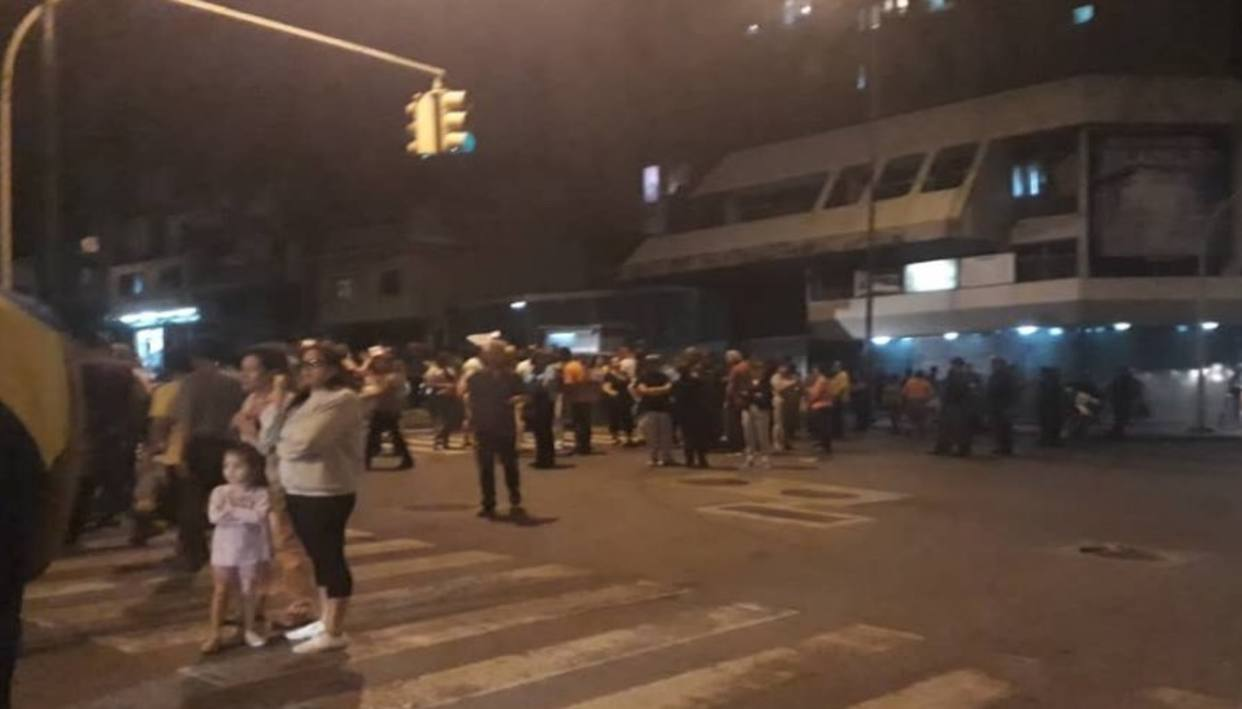
\includegraphics[width=300px]{35.jpg}%
\newline%
%
Vecinos de la avenida Baralt, ubicada en el municipio Libertador de Caracas, protestaron este lunes debido a la falta del suministro de agua potable.%
\newline%
%
Como medida de protesta, los ciudadanos obstaculizaron el paso en la vía,~~mientras sostenían pancartas exigiendo la restitución del servicio.%
\newline%
%
“Ciudadanos protestan en la avenida Baralt en el centro de Caracas ante la escasez de agua. Se presentan en el lugar efectivos de la PNB y de la GNB”, informó en Twitter la periodista Osmary Hernandez.%
\newline%
%
Al sitio se trasladaron~funcionarios de la Policía Nacional Bolivariana (PNB) y de la Guardia Nacional Bolivariana (GNB).%
\newline%
%
\end{document}